% \documentclass{article}
% %\usepackage[english]{babel}%
% \usepackage{graphicx}
% \usepackage{tabulary}
% \usepackage{tabularx}
% \usepackage[normalem]{ulem}
% \usepackage{cancel}
% \usepackage{tikz} 
% \usepackage{pdflscape}
% \usepackage{colortbl}
% \usepackage{lastpage}
% \usepackage{multirow}
% \usepackage{enumerate}
% \usepackage[shortlabels]{enumitem}
% \usepackage{color,soul}
% \usepackage{pdflscape}
% \usepackage{hyperref}
% %\usepackage[table]{xcolor}
% \usepackage{rotating}
% \usepackage{amsmath}
% \usepackage{fixltx2e}
% \usepackage{framed}
% \usepackage{mdframed}
% \usepackage[T1]{fontenc}
% \usepackage[utf8]{inputenc}
% \usepackage{textcomp}
% \usepackage{siunitx}
% \usepackage{ifthen}
% \usepackage{fancyhdr}
% \usepackage{gensymb}
% \usepackage{newunicodechar}
% \usepackage[document]{ragged2e}
% \usepackage[margin=1in,top=1.1in,headheight=57pt,headsep=0.1in]
% {geometry}
% \usepackage{ifthen}
% \usepackage{fancyhdr}
% \everymath{\displaystyle}
% \usepackage[document]{ragged2e}
% \usepackage{fancyhdr}
% \everymath{\displaystyle}
% \usepackage{empheq}

% \usepackage[most]{tcolorbox}

% \usepackage{booktabs} % Required for nicer horizontal rules in tables


% \usepackage{enumitem}

% %\usepackage[table,xcdraw]{xcolor}
% \usetikzlibrary{arrows}
% \linespread{2}%controls the spacing between lines. Bigger fractions means crowded lines%
% %\pagestyle{fancy}
% %\usepackage[margin=1 in, top=1in, includefoot]{geometry}
% %\everymath{\displaystyle}
% \linespread{1.3}%controls the spacing between lines. Bigger fractions means crowded lines%
% %\pagestyle{fancy}
% \pagestyle{fancy}
% \setlength{\headheight}{56.2pt}

% \definecolor{myblue}{rgb}{.8, .8, 1}
% \newcommand*\mybluebox[1]{%
% \colorbox{myblue}{\hspace{1em}#1\hspace{1em}}}

% \chead{\ifthenelse{\value{page}=1}{
\includegraphics[scale=0.3]{SCC}\\ \textbf \textbf Wastewater Constituents Analysis \& Laboratory Methods}}
% \rhead{\ifthenelse{\value{page}=1}{}{}}
% \lhead{\ifthenelse{\value{page}=1}{}{Wastewater Constituents Analysis \& Laboratory Methods}}
% \rfoot{\ifthenelse{\value{page}=1}{Module 1: WATR 048 - Spring 2019}{Module 1: WATR 048 - Spring 2019}}

% \lfoot{Shabbir Basrai}
% \cfoot{Page \thepage\ of \pageref{LastPage}}
% \renewcommand{\headrulewidth}{2pt}
% \renewcommand{\footrulewidth}{1pt}
% \begin{document}
% %\begin{empheq}[box=\mybluebox]{align}
% %a&=b\\
% %E&=mc^2 + \int_a^a x\, dx
% %\end{empheq}

% \newlist{steps}{enumerate}{1} % Defines "Steps" for enumerate as Step 1, Step 2 etc.
% \setlist[steps, 1]{label = Step \arabic*:} % Defines "Steps" for enumerate as Step 1, Step 2 etc.

% \setlist{nolistsep} % Reduce spacing between bullet points and numbered lists


%_______________________________________________________________________________________________________________________________________%
\chapterimage{Collections.jpg} % Chapter heading image

\chapter{Collections}

The collection system resembles a tree that branches out from the treatment plant to collect the wastewater from individual sources.

\section{Wastewater Collection Piping}\index{Wastewater Collection Piping}	
	\begin{itemize}
		\item A \hl{lateral} is the piping that connects the public sewer to the building. 
		\item Laterals flow into larger lines called \hl{mains}.
		\item Mains carry the flow into the largest lines in the system, called \hl{trunk lines}. 
		\item A trunk line is the pipe that brings water into the treatment plant.
	\end{itemize}
\section{Sanitary Sewer Systems}\index{Sanitary Sewer Systems}

Sanitary sewer systems collect and convey wastewater from residential, commercial and industrial sources to a centralized wastewater treatment facility for treatment. 

\subsection{Storm-water systems}\index{Storm-water systems}

Storm-water systems are designed solely for the conveyance of storm-waters waters directly to streams, rivers, lakes, or the ocean.
 
\subsection{Combined sewer systems}\index{Combined sewer systems}
\begin{itemize}
\item Combined sewer systems collect and convey sanitary sewage and urban runoff in a common piping system.
\item Combined sewers could potentially cause serious water pollution problems during combined sewer overflow (CSO) events when wet weather flows exceed the sewage treatment plant capacity.
	\end{itemize}
\begin{center}
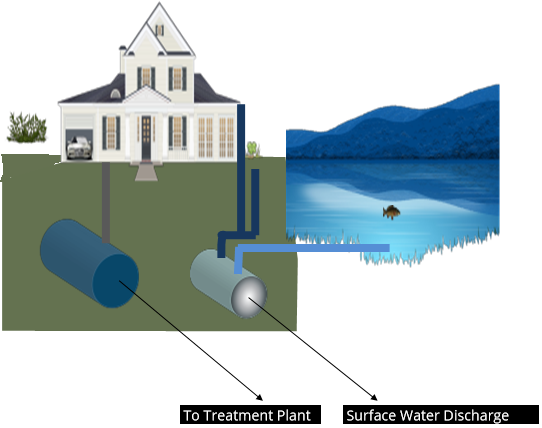
\includegraphics[scale=0.45]{SeperatedSystem1} \hspace{1 cm} 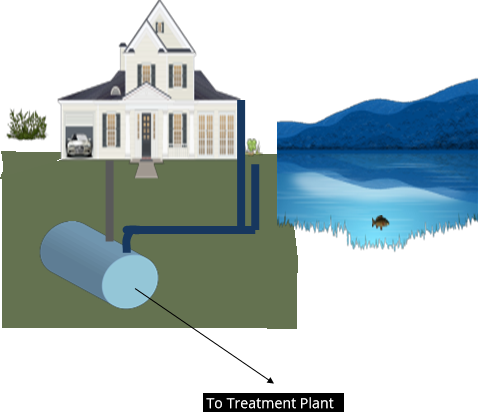
\includegraphics[scale=0.45]{CombinedSystem1}
\end{center}
			\hspace{2.6cm} Separated System \hspace{3.2cm} \parbox{\textwidth}{Combined System}\\

\section{Collections Systems Basics}\index{Collections Systems Basics}
	\begin{itemize}
\item The primary type of a collection system is a \hl{gravity system}. A gravity system is so named because the wastewater flows down gradient in the sewer, driven by forces of gravity. 
\item The collection system includes the gravity sewers, force mains, manholes, pumping equipment, and other facilities that collect and convey the water to a wastewater treatment plant. 
\item Sewers are generally laid at a minimum slope to ensure open channel flow through the pipe at a \hl{minimum velocity of 2.0 feet per second}. The minimum velocity is required to ensure that solids do not settle out in the sewer.  
\item When the sewer lines reach a certain depth, the flow must be lifted back through a lift or pump station.  
\item \hl{Lift stations} are built whenever wastewater must be pumped to a higher altitude, whether it's to lift water up so that it can gravity flow or to pump it over a rise or hill.  
\item The discharge from the pump station may be to another gravity sewer at that location or through a pressurized force main. 
\item Key elements of lift stations include a wastewater receiving well (wet-well), pumps and piping with associated valves.
\item The size of the wet well affects the operating of the station. If a wet well is too small, excessive starting and stopping of the pump motors will occur, resulting in premature failure. If the wet well is too large, solids will tend to settle on the bottom, blocking the pump suction line and leading to the generation of hydrogen sulfide and methane.
\item The dry well is the portion of the dry well/wet well pumping station that houses the necessary equipment required to pump the wastewater. The dry well is so named because it is isolated from the incoming wastewater.
\item Centrifugal pumps are the most common type of pump found in wastewater pumping stations. 
\item In the USA, wastewater generated in a typical home is about 70 gal/day/person
\end{itemize}

\section{Collections Related Operational Issues}\index{Collections Related Operational Issues}
Infiltration and inflow (I/I) is the unwanted flow into the wastewater collections systems.
\subsection{Infiltration}\index{Infiltration}
\begin{itemize} 
\item Groundwater entering sanitary sewers through defective pipe joints and broken pipes is called infiltration. \hl{Remember:  \textbf{ground filters}}
\end{itemize}

\subsection{Inflow}\index{Inflow}
\begin{itemize} 
\item During rainstorms or snow thaws, large volumes of water may flow into the wastewater collections systems through leaky manhole covers or combined storm-water /wastewater connections.  In addition, private residences may have roof, cellar, yard, area, or foundation drains inappropriately connected to sanitary sewers.  These flows are termed as inflows. \hl{Remember: \textbf{rain flow}}
\end{itemize}

\textbf{Implications of I/I:}\\%$$$$$$$$$$$$$$$$$$$$%
\begin{itemize}
\item I/I decrease the efficiency and capacity of wastewater collection systems and treatment systems 
\item I/I can advance the need for capital costs to manage and treat flows
\item I/I contribute to the hydraulic overloading of treatment processes, which can affect public health and the compliance with NPDES permit requirements
\item I/I could cause Sanitary and combined sewer overflows(SSOs and CSOs) when wastewater flow volumes exceed the design capacity of the treatment plant 
\item I/I increase collection system and treatment facility operating costs
\end{itemize}

\subsection{Odors}\index{Odors}
\begin{itemize}
\item Hydrogen sulfide (H$_2$S), its associated compounds and methane are generated due to microbial

 activity in wastewater and the conveyance systems.  The \hl{rotten egg like smell} of hydrogen sulfide causes public nuisance odors, poses a health hazard for collections systems workers and causes corrosion of the system through its conversion to sulfuric acid.  The hydrogen sulfide generation is typically controlled by reducing the potential for septicity in wastewater through proper design of the system -  adequate velocities and adequate air space and through chemical treatment.
 \end{itemize}

\subsection{Fats, Oils and Grease (FOG)}\index{Fats, Oils and Grease (FOG)}
\begin{itemize}
\item FOG from food home, food establishments and industries affect the operation of the collection system
\item FOG has a tendency to accumulate in sewer pipes decreasing its wastewater carrying capacity.
\item Excessive FOG accumulation may cause sewer overflows
 \end{itemize}

